\begin{frame}
	\myheading{Module 2.1: Biological Neurons}
\end{frame}

\begin{frame}
	\begin{columns}
		\column{0.5\textwidth}
		\begin{overlayarea}{\textwidth}{\textheight}
			\begin{figure}
				\centering
				  \begin{tikzpicture}

	\node (input0) at (9,-0.1)  {$x_{1}$};
	\node (input1) at (10,-0.1)  {$x_{2}$};
	\node (input2) at (11,-0.1)  {$x_{3}$};
	\node [hidden_neuron] (neuron1) at (10,2)  {$\sigma$};
	\node (output0)  at (10,3.5) {$y$};

	\draw [->] (input0) -- (neuron1);
	\draw [->] (input1) -- (neuron1);
	\draw [->] (input2) -- (neuron1);
	\draw [->] (neuron1) -- (output0);

	\node (formula)[scale=.8] at (9.1,0.6) {$w_{1}$};
	\node (formula)[scale=.8] at (9.8,0.6) {$w_{2}$};
	\node (formula)[scale=.8] at (10.4,0.6) {$w_{3}$};
  \end{tikzpicture}
				\caption{Artificial Neuron}
			\end{figure}
		\end{overlayarea}

		\column{0.5\textwidth}
		\begin{overlayarea}{\textwidth}{\textheight}
			\begin{itemize}\justifying
				\item<1-> The most fundamental unit of a deep neural network is called an \textit{artificial neuron}
				\item<2-> Why is it called a neuron ? Where does the inspiration come from ?
				\item<3-> The inspiration comes from biology (more specifically, from the \textit{brain})
				\item<4-> \textit{biological neurons = neural cells = neural processing units}
				\item<5-> We will first see what a biological neuron looks like ...
			\end{itemize}
		\end{overlayarea}
	\end{columns}
\end{frame}


\begin{frame}
	\begin{columns}
		\column{0.5\textwidth}
		\begin{overlayarea}{\textwidth}{\textheight}
				\begin{figure}
					\centering
					\includegraphics<1>[scale= 0.3]{images/module1/BioNeuron1.png}
					\includegraphics<2>[scale= 0.3]{images/module1/BioNeuron2.png}
					\includegraphics<3>[scale= 0.3]{images/module1/BioNeuron3.png}
					\includegraphics<4>[scale= 0.3]{images/module1/BioNeuron4.png}
					\includegraphics<5>[scale= 0.3]{images/module1/BioNeuron5.png}
					\caption{Biological Neurons$^*$\vspace{0.4in}\footnotetext{$^*$Image adapted from \url{https://cdn.vectorstock.com/i/composite/12,25/neuron-cell-vector-81225.jpg}}}
				\end{figure}
		\end{overlayarea}

		\column{0.5\textwidth}
		\begin{overlayarea}{\textwidth}{\textheight}
			\begin{itemize}\justifying
				\item<2-> \textbf{dendrite:} receives signals from other neurons
				\item<3-> \textbf{synapse:} point of connection to other neurons
				\item<4-> \textbf{soma:} processes the information
				\item<5-> \textbf{axon:} transmits the output of this neuron
			\end{itemize}
		\end{overlayarea}
	\end{columns}
\end{frame}


\begin{frame}
	\begin{columns}

		\column{0.5\textwidth}
		\begin{overlayarea}{\textwidth}{\textheight}
			\begin{figure}
				\centering
				\includegraphics<2>[scale= 0.5]{images/module1/SheldonExample2.png}
				\includegraphics<3>[scale= 0.5]{images/module1/SheldonExample3.png}
				\includegraphics<4>[scale= 0.5]{images/module1/SheldonExample4.png}
			\end{figure}
		\end{overlayarea}

		\column{0.5\textwidth}
		\begin{overlayarea}{\textwidth}{\textheight}
			\begin{itemize}\justifying
				\item<1-> Let us see a very cartoonish illustration of how a neuron works
				\item<2-> Our sense organs interact with the outside world
				\item<3-> They relay information to the neurons
				\item<4-> The neurons (may) get activated and produces a response (laughter in this case)

			\end{itemize}
		\end{overlayarea}
	\end{columns}
\end{frame}

\begin{frame}
	\begin{columns}

		\column{0.4\textwidth}
		\begin{overlayarea}{\textwidth}{\textheight}
			\begin{figure}
				\centering
				\includegraphics<1-3>[scale= 0.4]{images/module1/BigSheldonExample1.png}
				\includegraphics<4>[scale= 0.4]{images/module1/BigSheldonExample2.png}
				\includegraphics<5>[scale= 0.4]{images/module1/BigSheldonExample3.png}
				\includegraphics<6->[scale= 0.4]{images/module1/BigSheldonExample4.png}
			\end{figure}
		\end{overlayarea}

		\column{0.6\textwidth}
		\begin{overlayarea}{\textwidth}{\textheight}
			\begin{itemize}\justifying
				\item<1-> Of course, in reality, it is not just a single neuron which does all this
				\item<2-> There is a massively parallel interconnected network of neurons
				\item<3-> The sense organs relay information to the lowest layer of neurons
				\item<4-> Some of these neurons may fire (in red) in response to this information and in turn relay information to other neurons they are connected to
				\item<5-> These neurons may also fire (again, in red) and the process continues \onslide<6->{eventually resulting in a response (laughter in this case)}
				\item<7-> An average human brain has around $10^{11}$ (100 billion) neurons!
			\end{itemize}
		\end{overlayarea}
	\end{columns}
\end{frame}


\begin{frame}
	\begin{columns}
		\column{0.4\textwidth}
		\begin{overlayarea}{\textwidth}{\textheight}
			\begin{figure}
				\centering
				\includegraphics<1-2>[scale= 0.4]{images/module1/BigSheldonExample4.png}
				\includegraphics<3>[scale= 0.4]{images/module1/DivOfWork1.png}
				\includegraphics<4>[scale= 0.4]{images/module1/DivOfWork2.png}
				\includegraphics<5>[scale= 0.4]{images/module1/DivOfWork3.png}
				\includegraphics<6>[scale= 0.4]{images/module1/DivOfWork4.png}
				\includegraphics<7>[scale= 0.4]{images/module1/DivOfWork5.png}
				\only<3->{\caption{A simplified illustration}}
			\end{figure}
		\end{overlayarea}

		\column{0.6\textwidth}
		\begin{overlayarea}{\textwidth}{\textheight}
			\begin{itemize}\justifying
				\item<1-> This massively parallel network also ensures that there is division of work
				\item<2-> Each neuron may perform a certain role or respond to a certain stimulus

			\end{itemize}
		\end{overlayarea}
	\end{columns}
\end{frame}


\begin{frame}
	\begin{columns}
		\column{0.5\textwidth}
		\begin{overlayarea}{\textwidth}{\textheight}

			\begin{figure}
				\centering
				\includegraphics<2->[scale= 0.5]{images/module1/VisualCortex.png}
			\end{figure}
		\end{overlayarea}

		\column{0.5\textwidth}

		\begin{overlayarea}{\textwidth}{\textheight}

			\only<1-4>{
				\begin{itemize}\justifying
					\item<1-4> The neurons in the brain are arranged in a hierarchy
					\item<2-4> We illustrate this with the help of visual cortex (part of the brain) which deals with processing visual information
					\item<3-4> Starting from the retina, the information is relayed to several layers (follow the arrows)
					\item<4> We observe that the layers $V1$, $V2$ to $AIT$ form a hierarchy (from identifying simple visual forms to high level objects)
				\end{itemize}
			}

		\end{overlayarea}
	\end{columns}
\end{frame}

\begin{frame}
	\begin{columns}

		\column{0.5\textwidth}
		\begin{overlayarea}{\textwidth}{\textheight}

			\begin{figure}
				\centering
				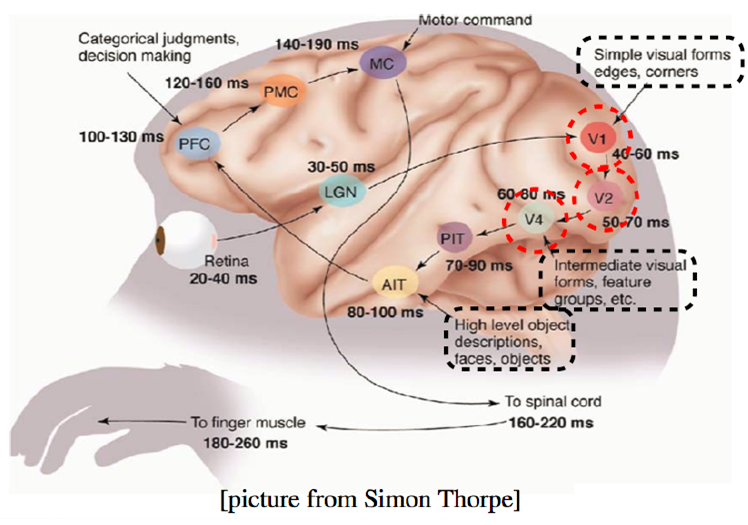
\includegraphics[scale= 0.5]{images/module1/VisualCortex.png}
			\end{figure}
		\end{overlayarea}

		\column{0.5\textwidth}

		\begin{overlayarea}{\textwidth}{\textheight}

			\onslide<1->{

				\begin{figure}
					\centering
					
\includegraphics[scale= 0.3]{images/module1/Layer1Rep.png}
				\end{figure}
			}

			\onslide<2->{
				\begin{figure}
					\centering
					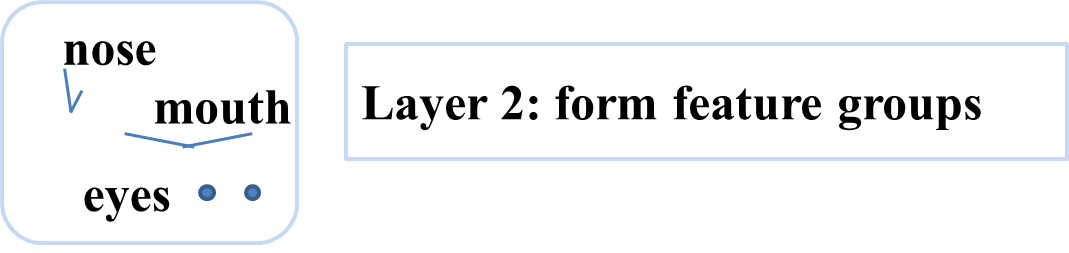
\includegraphics[scale= 0.3]{images/module1/Layer2Rep.png}
				\end{figure}
			}

			\onslide<3->{
				\begin{figure}
					\centering
					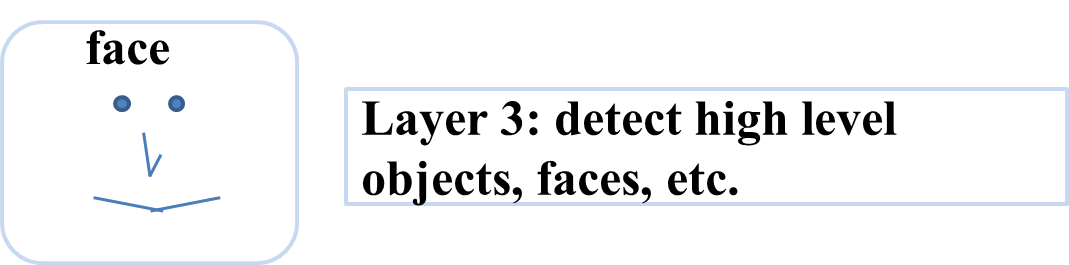
\includegraphics[scale= 0.3]{images/module1/Layer3Rep.png}
				\end{figure}
			}
			\onslide<1->{Sample illustration of hierarchical processing$^*$ \footnotetext{\hspace{-0.3in}$^*$Idea borrowed from Hugo Larochelle's lecture slides}}
		\end{overlayarea}
	\end{columns}
\end{frame}

\begin{frame}
	\begin{block}{Disclaimer}
		\begin{itemize}\justifying
			\item I understand very little about how the brain works!
			\item What you saw so far is an overly simplified explanation of how the brain works!
			\item But this explanation suffices for the purpose of this course!
		\end{itemize}
	\end{block}
\end{frame}
